\documentclass[../dissertation.tex]{subfiles}

\begin{document}

\section{Experiment 2}

Experiment 2 was an investigation in to whether the performance of ROS messages was affected by previous messages sent on the system. This was tested by comparing the performance of ROS messages of 5 consecutive message passing runs vs 5 message passing runs with system reboots between runs. This was repeated at 1KHz, 4KHz, 7KHz, and 10Khz frequencies for two reasons. The first was to investigate whether areas in which we observed consistent performance before would exhibit any difference between reboot and no reboot. Secondly, it would give further insight in to where the exact barrier between `good, consistent performance' and `poor, erratic performance' is.

Rebooting the systems involved has the opportunity to affect performance by stopping any background processes, interrupting slow processing messages from previous runs, and resetting any message caches and buffers in memory.

The result of the experiment was hypothesised to demonstrate no significant difference between rebooting and not-rebooting at any message frequency.

\begin{figure}[h]
\centering
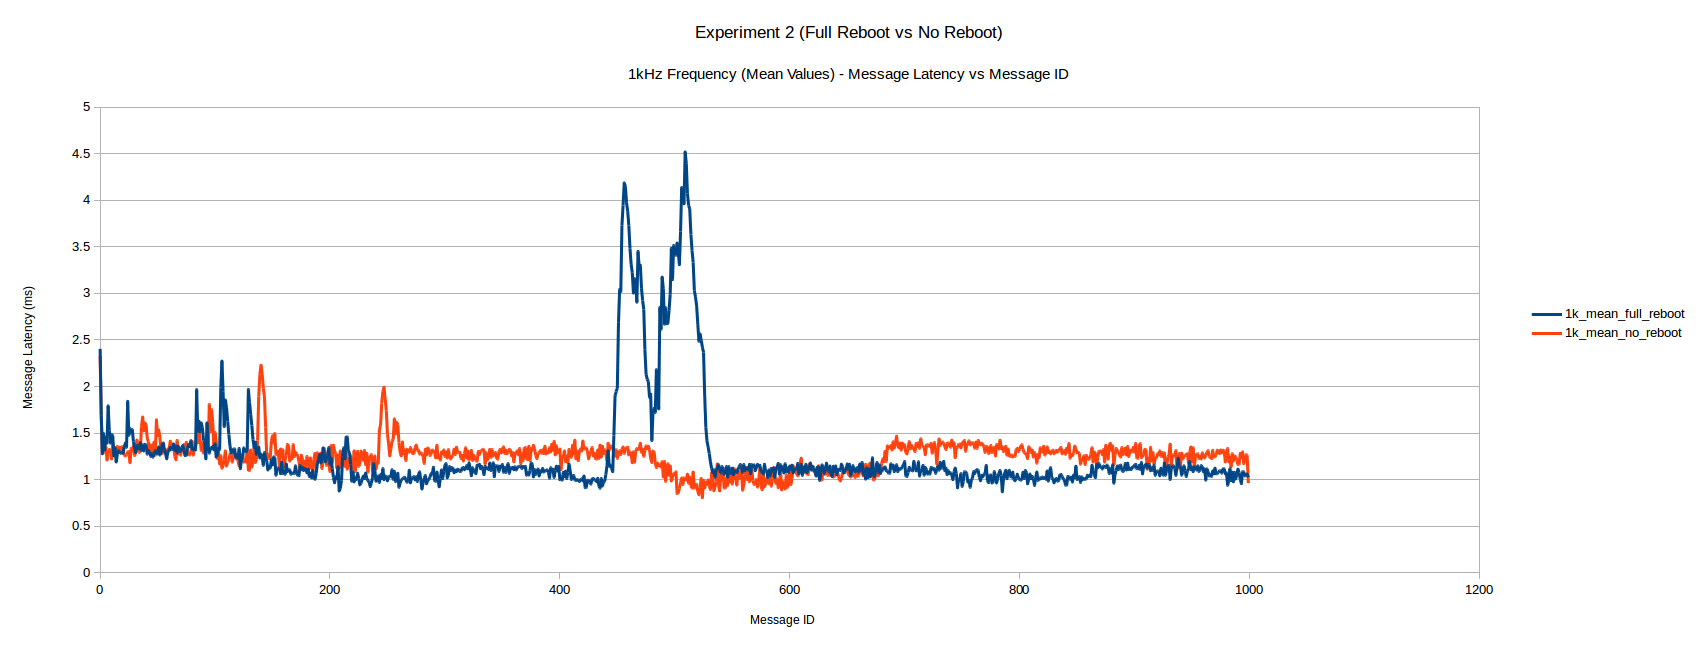
\includegraphics[width=\textwidth]{images/1khz-mean.png}
\caption{Experiment 2 - Mean Message Latency 1KHz Message Frequency}
\label{exp2-1khz-mean}
\end{figure}

Figure \ref{exp2-1khz-mean} demonstrates that for relatively low message frequencies the mean message latency was consistently 1 - 1.5ms (the peak around message 500 in the full reboot data was due to 1 erroneous run at that data point). Figure \ref{exp2-4khz-mean} is characteristic of the higher frequency runs - the no reboot runs generally gave equal or better performance compared to the full reboot runs. See Appendix \ref{exp2-appendix-results} for other mean graphs, and individual run graphs.

\begin{figure}[h]
\centering
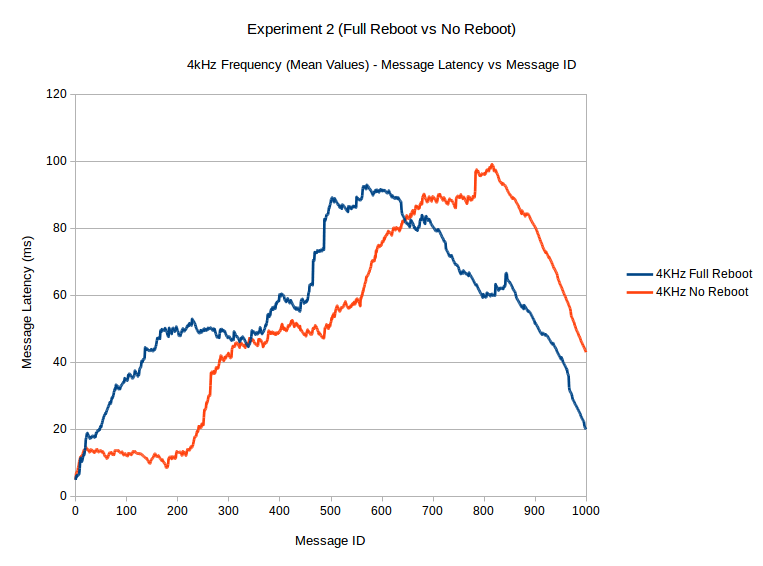
\includegraphics[width=\textwidth]{images/4khz-mean.png}
\caption{Experiment 2 - Mean Message Latency 4KHz Message Frequency}
\label{exp2-4khz-mean}
\end{figure}

\end{document}